\documentclass[tikz,border=7pt]{standalone}
\usepackage[utf8]{inputenc}
\usepackage[T1]{fontenc}
\usepackage{amsmath}
\usepackage{xcolor}
\usetikzlibrary{arrows.meta,positioning,calc}
\definecolor{brand}{HTML}{1E3A8A}
\definecolor{brandtwo}{HTML}{2563EB}
\definecolor{accentred}{HTML}{DC2626}
\definecolor{accentgreen}{HTML}{16A34A}
\definecolor{accentorange}{HTML}{F59E0B}
\definecolor{muted}{HTML}{64748B}
\definecolor{soft}{HTML}{EEF6FF}
\begin{document}
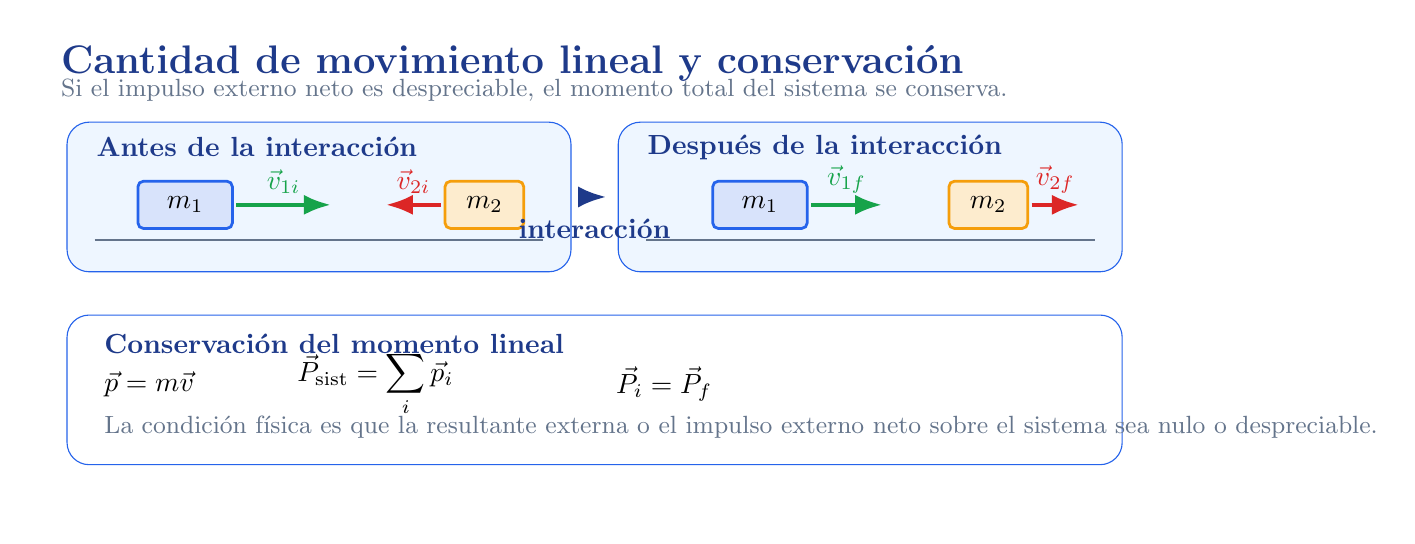
\begin{tikzpicture}[x=1cm,y=1cm,>=Latex]
  \fill[white] (-0.3,-0.4) rectangle (14.0,5.8);
  \node[anchor=west,text=brand,font=\bfseries\Large] at (0,5.35) {Cantidad de movimiento lineal y conservación};
  \node[anchor=west,text=muted,font=\small] at (0,5.0) {Si el impulso externo neto es despreciable, el momento total del sistema se conserva.};

  \draw[rounded corners=8pt,fill=soft,draw=brandtwo] (0.2,2.7) rectangle (6.6,4.6);
  \node[anchor=west,text=brand,font=\bfseries] at (0.45,4.28) {Antes de la interacción};
  \draw[thick,muted] (0.55,3.1)--(6.25,3.1);
  \draw[fill=brandtwo!18,draw=brandtwo,line width=1pt,rounded corners=2pt] (1.1,3.25) rectangle (2.3,3.85);
  \node at (1.7,3.55) {$m_1$};
  \draw[->,line width=1.5pt,accentgreen] (2.35,3.55)--(3.55,3.55) node[midway,above] {$\vec v_{1i}$};
  \draw[fill=accentorange!20,draw=accentorange,line width=1pt,rounded corners=2pt] (5.0,3.25) rectangle (6.0,3.85);
  \node at (5.5,3.55) {$m_2$};
  \draw[->,line width=1.5pt,accentred] (4.95,3.55)--(4.25,3.55) node[midway,above] {$\vec v_{2i}$};

  \draw[rounded corners=8pt,fill=soft,draw=brandtwo] (7.2,2.7) rectangle (13.6,4.6);
  \node[anchor=west,text=brand,font=\bfseries] at (7.45,4.28) {Después de la interacción};
  \draw[thick,muted] (7.55,3.1)--(13.25,3.1);
  \draw[fill=brandtwo!18,draw=brandtwo,line width=1pt,rounded corners=2pt] (8.4,3.25) rectangle (9.6,3.85);
  \node at (9.0,3.55) {$m_1$};
  \draw[->,line width=1.5pt,accentgreen] (9.65,3.55)--(10.55,3.55) node[midway,above] {$\vec v_{1f}$};
  \draw[fill=accentorange!20,draw=accentorange,line width=1pt,rounded corners=2pt] (11.4,3.25) rectangle (12.4,3.85);
  \node at (11.9,3.55) {$m_2$};
  \draw[->,line width=1.5pt,accentred] (12.45,3.55)--(13.05,3.55) node[midway,above] {$\vec v_{2f}$};

  \draw[->,line width=1.6pt,brand] (6.75,3.65)--(7.05,3.65);
  \node[text=brand,font=\bfseries] at (6.9,3.25) {interacción};

  \draw[rounded corners=8pt,fill=white,draw=brandtwo] (0.2,0.25) rectangle (13.6,2.15);
  \node[anchor=west,text=brand,font=\bfseries] at (0.55,1.78) {Conservación del momento lineal};
  \node[anchor=west] at (0.55,1.27) {$\vec p=m\vec v$};
  \node[anchor=west] at (3.0,1.27) {$\displaystyle \vec P_{\text{sist}}=\sum_i \vec p_i$};
  \node[anchor=west] at (7.05,1.27) {$\displaystyle \vec P_i=\vec P_f$};
  \node[anchor=west,text=muted,font=\small] at (0.55,0.72) {La condición física es que la resultante externa o el impulso externo neto sobre el sistema sea nulo o despreciable.};
\end{tikzpicture}
\end{document}